\section{Milestone M1: better gradients}
\label{sec:m1}

\begin{tcolorbox}[colback=gray!5, colframe=gray!40, title={M1 at a glance}, fonttitle=\bfseries]
  \textbf{Question.} Which gradient gives the most precision per shot?\quad
  \textbf{Answer.} RVB: ADAM with parameter shift (\VMIdealRvbPs{} without gate noise,
  \VMNoisyRvbPs{} with it). HVA: plain SPSA (\VMIdealHvaSpsa).\\
  \textbf{Code.} Commit \texttt{1a27c28}. \textbf{Results.} \py{results/m1_ideal-summary},
  \py{results/m1_noisy-summary}. \textbf{Status.} Done; three follow-ups open.
\end{tcolorbox}

\subsection{Goal and exit criteria}

The paper's ADAM runs used forward finite differences with step $\varepsilon=\VFdEps$. Under
shot noise such a difference divides noise by $\varepsilon$. M1 added an exact gradient
(parameter shift) and a two-energy hybrid, then compared all of them at an \emph{equal shot
budget}. Exit: a recommended default gradient per ansatz, recorded in the configs.

\subsection{Theory}

\begin{thm}[Parameter-shift rule \parencite{mitarai2018,schuld2019}]\label{thm:ps}
  Let $U(\theta)=e^{-i\theta G}$ with $G$ Hermitian, $G^2=\tfrac14 I$ (eigenvalues
  $\pm\tfrac12$), and $f(\theta)=\bra{\psi}V^\dagger U(\theta)^\dagger W^\dagger A\,W U(\theta)V\ket\psi$
  for fixed unitaries $V$, $W$ and an observable $A$. Then for every $\theta$,
  \[
    f'(\theta)=\tfrac12\bigl[f(\theta+\tfrac\pi2)-f(\theta-\tfrac\pi2)\bigr].
  \]
\end{thm}

\begin{proof}
  Because $(2G)^2=I$, $U(\theta)=\cos\tfrac\theta2\,I-i\sin\tfrac\theta2\,(2G)$. Substituting,
  $f$ is a quadratic form in $(\cos\frac\theta2,\sin\frac\theta2)$, hence a trigonometric
  polynomial of degree one: $f(\theta)=a+b\cos\theta+c\sin\theta$ for constants $a,b,c$. Then
  $f(\theta\pm\tfrac\pi2)=a\mp b\sin\theta\pm c\cos\theta$, and the half-difference is
  $-b\sin\theta+c\cos\theta=f'(\theta)$.
\end{proof}

Both ansatzes qualify gate by gate. Each eSWAP is $e^{-i\phi\,\SWAP/2}$, and $G=\SWAP/2$ has
eigenvalues $\pm\frac12$. Each HVA rotation $R_{PP}(\theta)=e^{-i\theta\,PP/2}$ has $G=PP/2$.
The legacy eSWAP contains a controlled rotation, whose generator has three eigenvalues; it
would need a four-term rule and is not supported.

\begin{cor}[Shared parameters]\label{cor:shared}
  If a parameter $\theta_j$ drives $K_j$ such gates, then
  $\partial_{\theta_j}E=\sum_{k=1}^{K_j}\tfrac12\bigl[E(\varphi+\tfrac\pi2e_k)-E(\varphi-\tfrac\pi2e_k)\bigr]$
  evaluated at the \emph{unshared} vector $\varphi=\mathrm{expand}(\theta)$, which has one entry
  per occurrence. One gradient costs $2\sum_jK_j$ energies: $\VPsEnergiesRvb$ for RVB ($K_j=1$)
  and $\VPsEnergiesHva$ for HVA ($K_j=18$).
\end{cor}

\begin{proof}
  The energy is $E(\theta)=F(\mathrm{expand}(\theta))$ where $F$ treats occurrences as
  independent. By the chain rule, $\partial_{\theta_j}E=\sum_{k:\,k\mapsto j}\partial_{\varphi_k}F$,
  and each term is given by \cref{thm:ps} with $V,W$ the rest of the circuit.
\end{proof}

A single shift of a shared HVA parameter does \emph{not} work: the summed generator
$\sum_kG_k$ has many eigenvalues, so $E$ is a higher-degree trigonometric polynomial in
$\theta_j$. The package implements \cref{cor:shared} with \py{unshare_parameters}, which rewrites
the circuit with one parameter per occurrence and returns a \py{ParameterMap} with
\py{expand} ($\theta\mapsto\varphi$) and \py{contract} (sum of occurrence gradients). The
unshared circuit prepares the same state and transpiles to the same \VCxHvaUnshared{} CX
(Table~\ref{tab:circuits}).

\begin{prop}[Gradient noise per component]\label{prop:gradnoise}
  Suppose every energy estimate carries independent noise of standard deviation $\sigma$. The
  per-component noise of the gradient estimate is
  \[
    \text{forward: }\frac{\sqrt2\,\sigma}{\varepsilon},\qquad
    \text{central: }\frac{\sqrt2\,\sigma}{2\varepsilon},\qquad
    \text{parameter shift: }\sigma\sqrt{K_j/2}.
  \]
  At an equal budget $B$ of shots per iteration split over $m$ energies, $\sigma=\sigma_B\sqrt m$,
  where $\sigma_B$ is the noise of one energy measured with all $B$ shots.
\end{prop}

\begin{proof}
  Forward: $(\hat E(\theta+\varepsilon e_j)-\hat E(\theta))/\varepsilon$ has variance
  $2\sigma^2/\varepsilon^2$. Central: $(\hat E_+-\hat E_-)/(2\varepsilon)$ has variance
  $2\sigma^2/(4\varepsilon^2)$. Parameter shift: a sum of $K_j$ half-differences, each with variance
  $2\sigma^2/4$, gives $K_j\sigma^2/2$. Shot noise scales as $1/\sqrt{\text{shots}}$, and each
  of the $m$ energies gets $B/m$ shots, so $\sigma=\sigma_B\sqrt m$.
\end{proof}

With $\varepsilon=\VFdEps$ the forward difference amplifies noise \VSigmaFwd-fold at fixed shots
per energy, while parameter shift gives \VSigmaPsRvb$\sigma$ for RVB. At equal budget
(Table~\ref{tab:m1}) the picture sharpens: for RVB parameter shift wins by an order of magnitude
(\VBudgetPsRvb$\sigma_B$ against \VBudgetFwdRvb$\sigma_B$), but for HVA its 72 energies cancel the
advantage (\VBudgetPsHva$\sigma_B$ against \VBudgetFwdHva$\sigma_B$). Finite differences are
also biased, by $O(\varepsilon)$ for forward and $O(\varepsilon^2)$ for central; parameter shift is
unbiased.

\begin{dfn}[SPSA and the hybrid]
  SPSA \parencite{spall1992} draws a random sign vector $\Delta\in\{\pm1\}^n$ and estimates
  $\hat g=\Delta\,[E(\theta+c\Delta)-E(\theta-c\Delta)]/(2c)$ from two energies, whatever $n$.
  \emph{Plain SPSA} takes the step $\theta\leftarrow\theta-a\,\hat g$ with a \VSpsaCalibrated{}
  gain $a=\VSpsaLr$ in M1. The \emph{hybrid} feeds the same two-energy estimate into ADAM
  \parencite{kingma2014}, whose step $-\eta\,\hat m/(\sqrt{\hat v}+\epsilon)$ divides the averaged
  gradient $\hat m$ by its running root-mean-square $\sqrt{\hat v}$.
\end{dfn}

\subsection{Protocol}

Every method spends the same \VMBudget{} shots per measurement basis per iteration, split evenly
over the $m$ energies its gradient needs. All gradient methods share ADAM with learning rate
$\VAdamLr$, so differences come from the gradients alone; plain SPSA is the baseline. The metric
is the \emph{ideal} energy of the final parameters (\cref{sec:pipeline}): how good the parameters
are, separately from the noise floor. Two settings:
\begin{itemize}
  \item shot noise only (\py{aer_ideal}), \VMItersHva{} iterations, \VMSeeds{} seeds, both
    ansatzes (\py{configs/m1_gradients_ideal.toml});
  \item full \py{FakeGuadalupeV2} noise, \VMNoisyIters{} iterations, one seed, RVB only, because
    noisy simulation costs about \VSecPerEnergy{}\,s per energy and HVA parameter shift needs 72
    energies per step (\py{configs/m1_gradients_noisy.toml}).
\end{itemize}

\subsection{Results}

\begin{table}[H]
  \centering
  \footnotesize
  \setlength{\tabcolsep}{4pt}
  % Generated by `uv run python -m docsgen`; do not edit.
\begin{tabular}{llccccc}
\toprule
 &  &  & \multicolumn{2}{c}{gradient noise per component} & \multicolumn{2}{c}{noise-free error of final parameters} \\
\cmidrule(lr){4-5}\cmidrule(lr){6-7}
ansatz & method & $m$ & fixed shots ($\sigma$) & equal budget ($\sigma_B$) & shot noise (\VMSeeds{} seeds) & device noise (1 seed) \\
\midrule
HVA & ADAM, forward differences (paper) & \VMEnergiesHvaFwd & \VSigmaFwd & \VBudgetFwdHva & \VMIdealHvaFwd ${}\pm{}$ \VMIdealHvaFwdSd & not run \\
 & ADAM, central differences & \VMEnergiesHvaCen & \VSigmaCen & \VBudgetCenHva & \VMIdealHvaCen ${}\pm{}$ \VMIdealHvaCenSd & not run \\
 & ADAM, SPSA gradient (hybrid) & \VMEnergiesHvaHyb & -- & -- & \VMIdealHvaHyb ${}\pm{}$ \VMIdealHvaHybSd & not run \\
 & ADAM, parameter shift & \VMEnergiesHvaPs & \VSigmaPsHva & \VBudgetPsHva & \VMIdealHvaPs ${}\pm{}$ \VMIdealHvaPsSd & not run \\
 & plain SPSA & \VMEnergiesHvaSpsa & -- & -- & \VMIdealHvaSpsa ${}\pm{}$ \VMIdealHvaSpsaSd & not run \\
\midrule
RVB & ADAM, forward differences (paper) & \VMEnergiesRvbFwd & \VSigmaFwd & \VBudgetFwdRvb & \VMIdealRvbFwd ${}\pm{}$ \VMIdealRvbFwdSd & \VMNoisyRvbFwd \\
 & ADAM, central differences & \VMEnergiesRvbCen & \VSigmaCen & \VBudgetCenRvb & \VMIdealRvbCen ${}\pm{}$ \VMIdealRvbCenSd & not run \\
 & ADAM, SPSA gradient (hybrid) & \VMEnergiesRvbHyb & -- & -- & \VMIdealRvbHyb ${}\pm{}$ \VMIdealRvbHybSd & \VMNoisyRvbHyb \\
 & ADAM, parameter shift & \VMEnergiesRvbPs & \VSigmaPsRvb & \VBudgetPsRvb & \VMIdealRvbPs ${}\pm{}$ \VMIdealRvbPsSd & \VMNoisyRvbPs \\
 & plain SPSA & \VMEnergiesRvbSpsa & -- & -- & \VMIdealRvbSpsa ${}\pm{}$ \VMIdealRvbSpsaSd & \VMNoisyRvbSpsa \\
\bottomrule
\end{tabular}

  \caption{Equal-budget gradient comparison. $m$: energies per iteration, read from the
    evaluation counts of the runs. Gradient noise from \cref{prop:gradnoise}. Errors are the
    noise-free relative error of the final parameters: mean $\pm$ sample standard deviation
    over seeds.\protect\footnotemark}
  \label{tab:m1}
\end{table}
\footnotetext{Sample standard deviation ($\mathrm{ddof}=1$). The README's M1 table originally used
the population value ($\mathrm{ddof}=0$), smaller by $\sqrt{4/5}$ for five seeds; \py{main} switched it to the sample value in
\texttt{687d0ae}. The means agree, and \py{docsgen/tests} checks them.}

\begin{figure}[H]
  \centering
  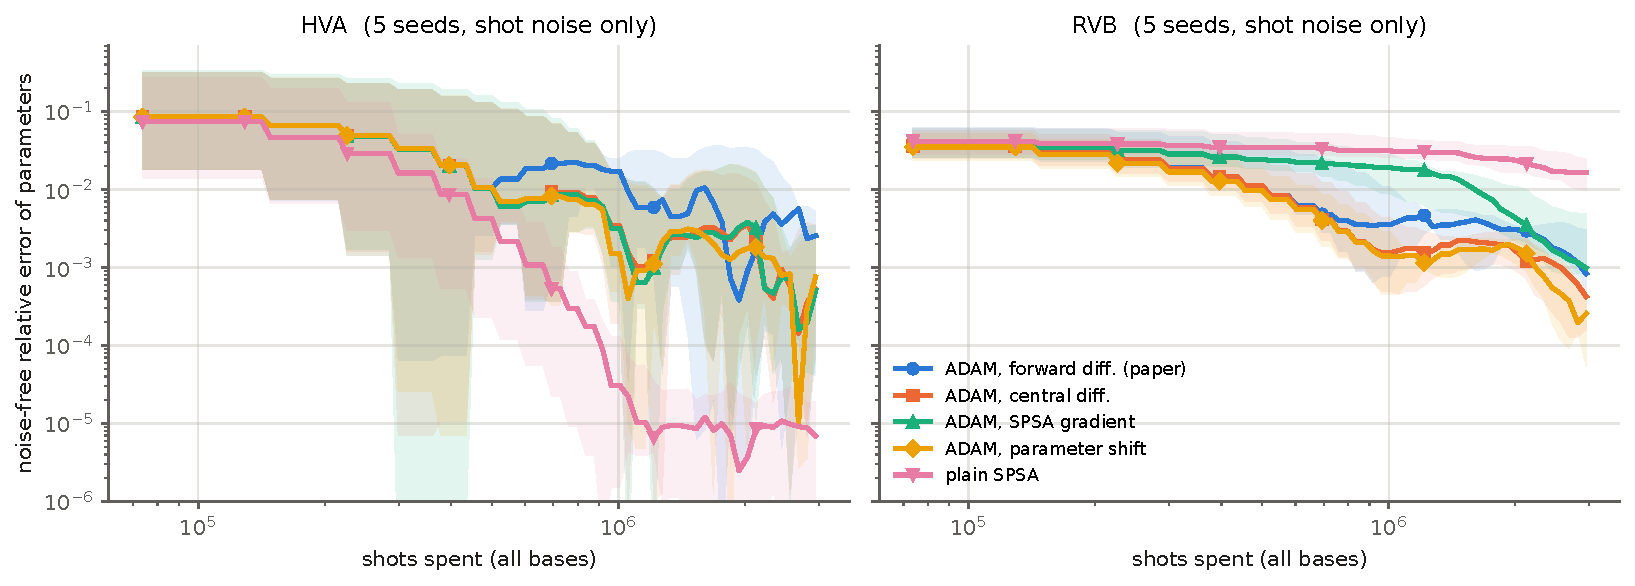
\includegraphics[width=\linewidth]{m1_ideal_vs_shots}
  \caption{Noise-free relative error of the current parameters against shots spent (all bases),
    shot noise only. Line: median over seeds; band: min--max. The same metric as
    \py{kagome_vqe.plotting.plot_ideal_vs_shots}, coloured by method consistently across this
    report and the slides.}
  \label{fig:m1curves}
\end{figure}

\begin{figure}[H]
  \centering
  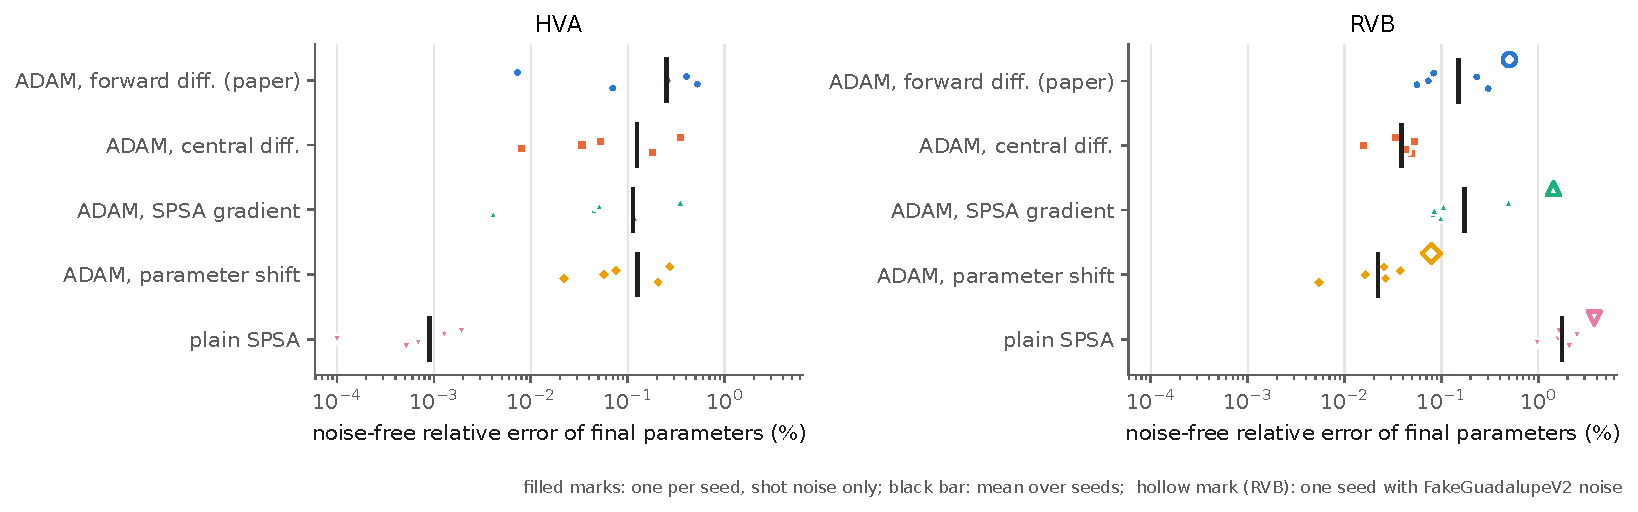
\includegraphics[width=\linewidth]{m1_final}
  \caption{Final noise-free error per method. Filled marks: one per seed (shot noise only); black
    bar: mean. Hollow marks (RVB): the single seed with device noise.}
  \label{fig:m1final}
\end{figure}

Figures~\ref{fig:m1curves} and~\ref{fig:m1final} support three readings.
\begin{enumerate}
  \item \textbf{RVB: parameter shift is best} with and without device noise
    (\VMIdealRvbPs{} and \VMNoisyRvbPs{}), against \VMIdealRvbFwd{} and \VMNoisyRvbFwd{} for the
    paper's forward differences. This matches \cref{prop:gradnoise}: at equal budget its
    per-component noise is an order of magnitude lower. Plain SPSA is the least precise for RVB's
    12 parameters (\VMIdealRvbSpsa), and its two-energy estimate is a poor direction in 12
    dimensions.
  \item \textbf{HVA: plain SPSA is best} by two orders of magnitude (\VMIdealHvaSpsa), while
    every ADAM variant, \emph{whatever its gradient}, ends near $0.1\,\%$. Identical plateaus
    for gradients of very different quality point to the update rule, not the gradient. Near the
    minimum the true gradient vanishes but the noise does not, so $\sqrt{\hat v}$ tracks the noise
    and ADAM's normalised step stays of order $\eta=\VAdamLr$ per component: it keeps jittering
    around the minimum. Plain SPSA's step $a\hat g$ shrinks in mean with the gradient. HVA has
    only two parameters, so SPSA's random directions lose little.
  \item \textbf{Noise floor unchanged.} The re-measured noisy energies of the M1 runs stay at the
    floor of \cref{sec:noise} (\VMNoisyFinalRvbPs{} for parameter shift): better gradients
    improve the parameters, not what the device reads.
\end{enumerate}

\subsection{Problems solved and open}

\begin{itemize}
  \item[\checkmark] Parameter shift matches finite differences without noise to about
    $10^{-9}$ for HVA, RVB and \py{real_amplitudes}; energy counts 24 and 72 are unit-tested.
  \item[\checkmark] Defaults recorded: \py{configs/fake_guadalupe_rvb_adam_ps.toml} (RVB, ADAM +
    parameter shift) and \py{configs/ibm_hva_spsa.toml} (HVA, SPSA).
  \item[$\circ$] \textbf{ADAM's step size limits HVA.} A decaying learning rate should be tried
    before concluding that SPSA is intrinsically better for HVA.
  \item[$\circ$] \textbf{RVB had not converged} when the budget ran out
    (Figure~\ref{fig:m1curves}, right: curves still falling at three million shots); longer runs
    may reorder the close finishers.
  \item[$\circ$] \textbf{The noisy check used one seed.} Repeat with more seeds before relying on
    the smaller differences (e.g.\ forward against central).
\end{itemize}

\subsection*{Exercises}

\begin{exer}
  With $\varepsilon=0.1$, how many times more shots per energy does a forward difference need to
  match the per-component noise of parameter shift on RVB?
\end{exer}
\begin{sol}
  Equate $\sqrt2\sigma_1/0.1=\sigma_2/\sqrt2$: $\sigma_1/\sigma_2=0.05$, so $1/0.05^2=400$ times
  more shots per energy. With 13 instead of 24 energies per gradient, the total shot cost is still
  about $400\times13/24\approx217$ times higher.
\end{sol}

\begin{exer}
  Show that a single symmetric shift of a shared HVA parameter, $\tfrac12[E(\theta_j+\tfrac\pi2)-E(\theta_j-\tfrac\pi2)]$,
  is \emph{not} the derivative in general.
\end{exer}
\begin{sol}
  With $K$ gates sharing $\theta_j$, $E$ is a trigonometric polynomial of degree up to $K$ in
  $\theta_j$ (each gate contributes degree one). The two-term rule is exact only for degree one;
  for example $E=\cos2\theta$ gives $\tfrac12[\cos(2\theta+\pi)-\cos(2\theta-\pi)]=0\neq-2\sin2\theta$.
\end{sol}
